% 1) Title
% 2) Date
% 3) Location
% 4) Present
% 5) Picture
% 6) Start Time
% 7) Stop Time
\insertmeeting 
	{Team Time} 
	{08/10/21}
	{Hagerty High School}
	{Annika, Anouska, Clayton, Falon, James, Jensen, Nathan, Ritam, Rose, Samantha}
	{Images/RobotPics/robot.jpg}
	{2:20}
  {4:30}
	
\section*{General}
\noindent\hfil\rule{\textwidth}{.4pt}\hfil
\subsection*{Goals}
\begin{itemize}
    \item Set up goals for the season
	\item Discuss GRPI model

\end{itemize} 

\noindent\hfil\rule{\textwidth}{.4pt}\hfil

\subsection*{Accomplishments}
At today's meeting, we went over the GRPI model --- a type of model that helps teams work together more effectively. GRPI stands for goals, roles, processes, and interpersonal relations. This model is designed to help teams asses and organize tasks. At this meeting, we started discussing our overall goals and creating a list of what each goal would entail (image 1) these goals encompassed everything we wanted to accomplish this season including having a fully functioning robot, having a well made notebook, reaching out to more professionals, expanding our outreach, creating an innovation project, and finally progressing to worlds. 
We also discussed our committees and what roles each of them would take. We used a chart organizing us into our main (blue) and secondary(gray) committees and allowed people to change their selections if desired (image 2). Additionally, we went over what each of these committees roles would be and what responsibilities its members would have, utilizing notes from a previous meeting and adding details and making changes where it was necessary(see images 3 and 4).

\begin{figure}[htp]
\centering
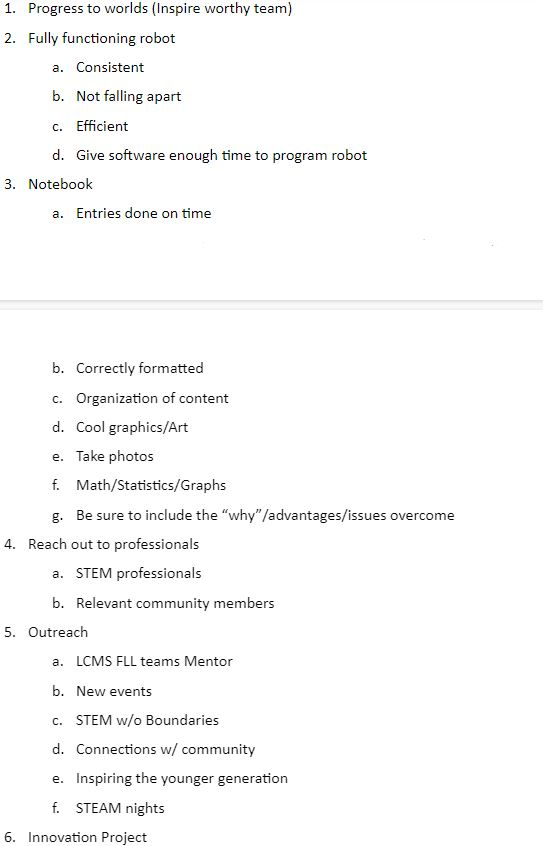
\includegraphics[width=0.9\textwidth, angle=0]{Meetings/August/08-10-21/8-10-21_Image1 - Nathan Forrer.JPG}
\caption{Plan for the season}
\label{fig:pic1}
\end{figure}

\begin{figure}[ht]
\centering
\begin{minipage}[b]{.50\textwidth}
	\centering
	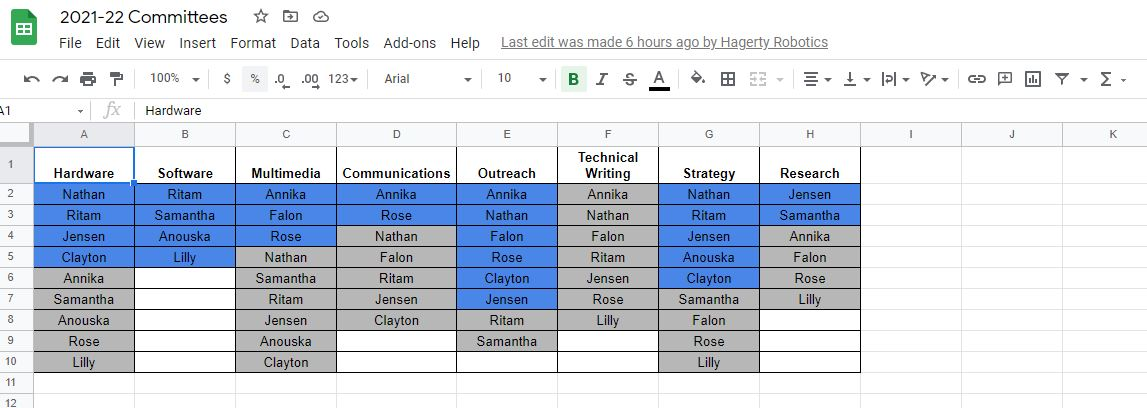
\includegraphics[width=0.8\textwidth, angle=0]{Meetings/August/08-10-21/8-10-21_Image2 - Nathan Forrer.JPG}
	\caption{Committee Division Sheet}
	\label{fig:pic2}
\end{minipage}%
\hfill%
\begin{minipage}[b]{.50\textwidth}
	\centering
	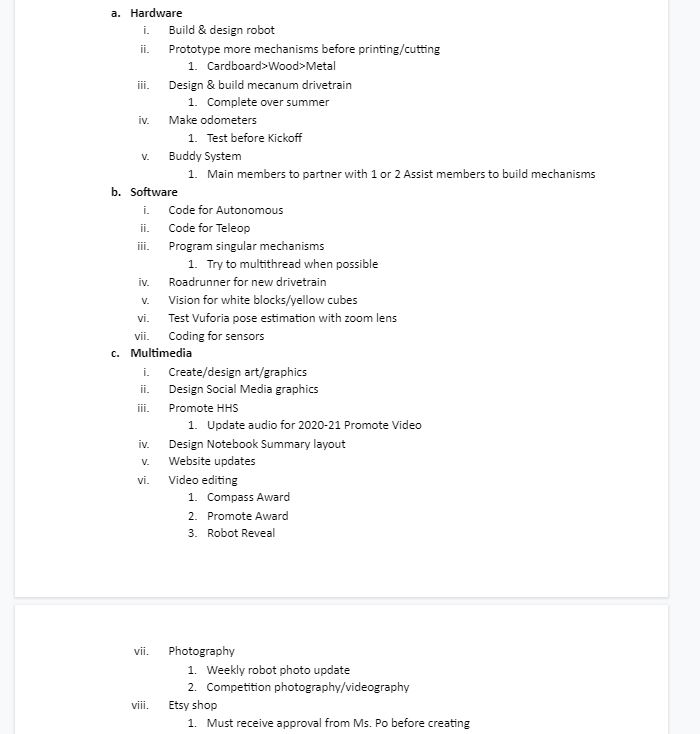
\includegraphics[width=0.8\textwidth, angle=0]{Meetings/August/08-10-21/8-10-21_Image3 - Nathan Forrer.JPG}
	\caption{Committee Goals Sheet}
	\label{fig:pic3}
\end{minipage}
\end{figure}

\begin{figure}[htp]
\centering
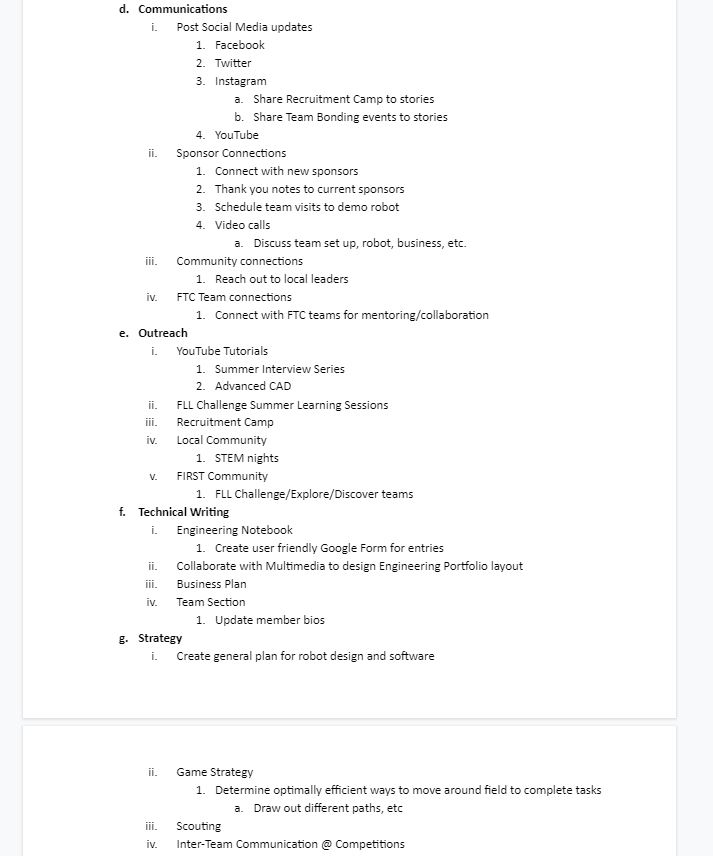
\includegraphics[width=0.9\textwidth, angle=0]{Meetings/August/08-10-21/8-10-21_Image4 - Nathan Forrer.JPG}
\caption{Committee Goals Sheet Continued}
\label{fig:pic4}
\end{figure}